\section{Kiến trúc hệ thống và Công nghệ sử dụng}

\subsection{Ngôn ngữ lập trình C++}

Trò chơi được viết hoàn toàn bằng \textbf{C++}, ngôn ngữ biên dịch do Bjarne Stroustrup phát triển từ C, có bổ sung lập trình hướng đối tượng. Nhóm chọn C++ vì các lý do sau:

\begin{itemize}
    \item \textbf{Hiệu năng cao}: mã được biên dịch thẳng ra mã máy, vòng lặp trò chơi chạy khoảng 33 khung hình mỗi giây mà gần như không tốn CPU.
    \item \textbf{Hỗ trợ hướng đối tượng}: lớp, kế thừa và đa hình qua hàm ảo giúp mô hình hóa 7 loại khối Tetromino một cách tự nhiên. Mỗi loại khối là một lớp con có hình dạng và cách xoay riêng.
    \item \textbf{Kiểm soát bộ nhớ}: khối gạch được cấp phát bằng \texttt{new} và giải phóng bằng \texttt{delete}. Nhờ vậy nhóm được thực hành quản lý vòng đời đối tượng.
    \item \textbf{Quen thuộc với cả nhóm}: đây là ngôn ngữ cả nhóm đã học ở các môn lập trình cơ bản, nên thành viên nào cũng đọc hiểu và đóng góp được.
\end{itemize}

Mã nguồn dùng một số tính năng của chuẩn \textbf{C++11}, như \texttt{nullptr} (con trỏ rỗng có kiểu) và \texttt{override} (đánh dấu hàm ghi đè hàm ảo). Vì vậy chương trình phải được biên dịch với chuẩn C++11 trở lên.

\subsection{Môi trường phát triển và Thư viện}

Nhóm lập trình trên \textbf{Visual Studio Code}, biên dịch bằng \textbf{G++ (MinGW-w64)} trên Windows 10/11, quản lý mã nguồn bằng \textbf{Git/GitHub} (mỗi thành viên làm trên nhánh riêng và gộp mã qua Pull Request), và soạn báo cáo bằng \LaTeX. Trò chơi không dùng thư viện đồ họa bên ngoài, chỉ dùng thư viện chuẩn C++ và thư viện có sẵn của Windows (Bảng~\ref{tab:thu_vien}).

\begin{table}[H]
    \centering
    \caption{Các thư viện được sử dụng và vai trò}
    \label{tab:thu_vien}
    \renewcommand{\arraystretch}{1.35}
    \begin{tabularx}{\textwidth}{|p{3cm}|X|}
        \hline
        \textbf{Thư viện} & \textbf{Vai trò trong trò chơi} \\
        \hline
        \texttt{<iostream>} & Xuất bảng chơi, điểm số, cấp độ và các màn hình thông báo ra console. \\
        \hline
        \texttt{<conio.h>} & Nhận phím không chặn: kiểm tra có phím đang chờ không, và đọc phím mà không cần nhấn Enter. Nhờ vậy khối vẫn rơi khi người chơi không bấm gì. \\
        \hline
        \texttt{<windows.h>} & Tạm dừng giữa các khung hình, chuyển console sang UTF-8, bật xử lý mã màu ANSI và ẩn con trỏ nhấp nháy. \\
        \hline
        \texttt{<cstdlib>}, \texttt{<ctime>} & Sinh số ngẫu nhiên để xáo trộn túi khối, lấy thời gian hiện tại làm hạt giống để mỗi ván có thứ tự khối khác nhau, và gọi lệnh xóa màn hình. \\
        \hline
    \end{tabularx}
\end{table}

Vì phụ thuộc \texttt{<conio.h>} và \texttt{<windows.h>}, phiên bản hiện tại chỉ chạy được trên Windows.

\subsection{Sơ đồ kiến trúc tổng quan (Architecture Overview)}

Chương trình là một ứng dụng console chạy một luồng, toàn bộ mã nằm trong tệp \texttt{tetris/main.cpp}. Về mặt logic, mã được chia thành các thành phần có trách nhiệm riêng như Hình~\ref{fig:kien_truc_tong_quan}.

\begin{figure}[H]
    \centering
    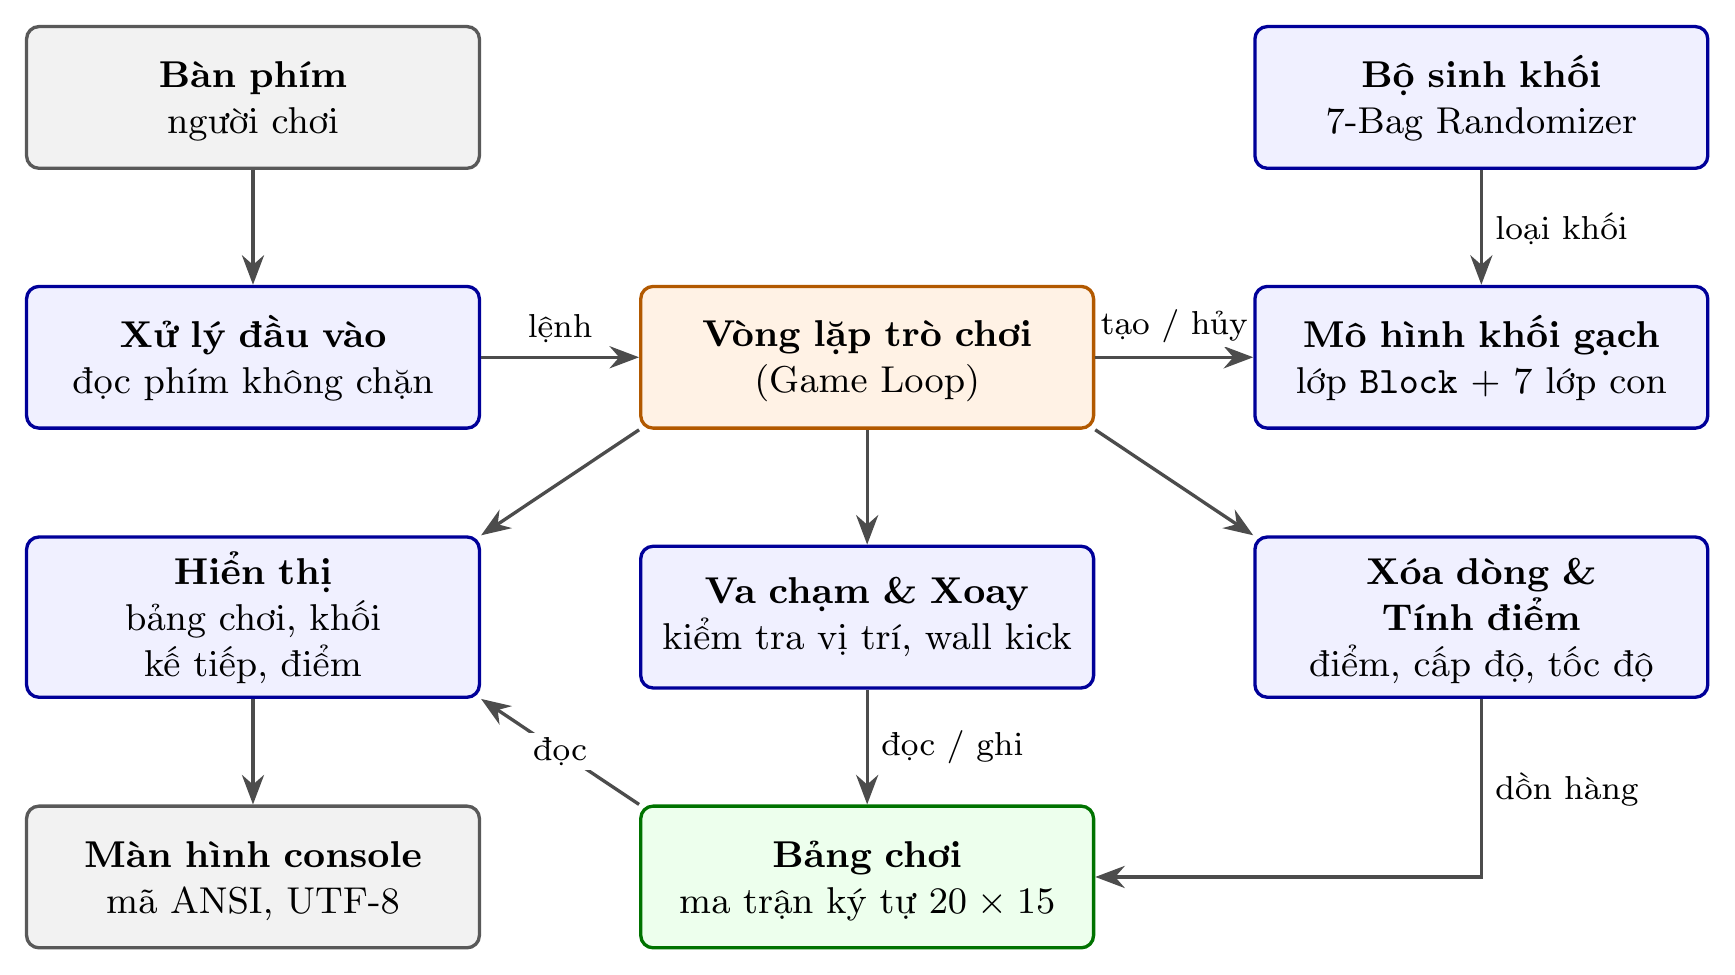
\includegraphics[width=0.85\textwidth]{04_tai_lieu_ky_thuat/so_do/kien_truc_tong_quan.png}
    \caption{Sơ đồ kiến trúc tổng quan của trò chơi}
    \label{fig:kien_truc_tong_quan}
\end{figure}

\begin{itemize}
    \item \textbf{Vòng lặp trò chơi} là trung tâm điều phối. Nó giữ trạng thái ván chơi và gọi các thành phần khác theo thứ tự cố định trong mỗi khung hình.
    \item \textbf{Xử lý đầu vào} đọc mọi phím đang chờ và chuyển thành lệnh: trái, phải, rơi nhanh, xoay, thả thẳng, tạm dừng, thoát.
    \item \textbf{Bộ sinh khối} và \textbf{mô hình khối gạch} quyết định khối tiếp theo và lưu hình dạng, cách xoay của từng loại khối (Mục~\ref{subsec:7bag}).
    \item \textbf{Va chạm \& Xoay} và \textbf{Xóa dòng \& Tính điểm} là các thuật toán đọc và ghi lên \textbf{bảng chơi}. Bảng chơi là ma trận ký tự dùng chung, là nguồn dữ liệu duy nhất cho cả logic lẫn hiển thị.
    \item \textbf{Hiển thị} đưa con trỏ về góc trên bên trái rồi vẽ đè lên khung hình cũ thay vì xóa màn hình, nhờ đó hạn chế nhấp nháy. Mỗi loại khối có một màu ANSI riêng.
\end{itemize}

\subsection{Luồng hoạt động chính của Game Loop}
\label{subsec:game_loop}

Hàm \texttt{main} có hai vòng lặp lồng nhau. \textbf{Vòng lặp ngoài} quản lý phiên chơi. Nó đặt lại điểm, cấp độ, tốc độ, túi khối và bảng chơi, rồi bắt đầu ván mới. Khi ván kết thúc, nó hiện màn hình \textit{Game Over} để người chơi chọn chơi lại (\texttt{R}) hoặc thoát (\texttt{Q}). \textbf{Vòng lặp trong} là game loop thực sự, mỗi vòng là một khung hình khoảng 30\,ms (Hình~\ref{fig:game_loop}).

\begin{figure}[H]
    \centering
    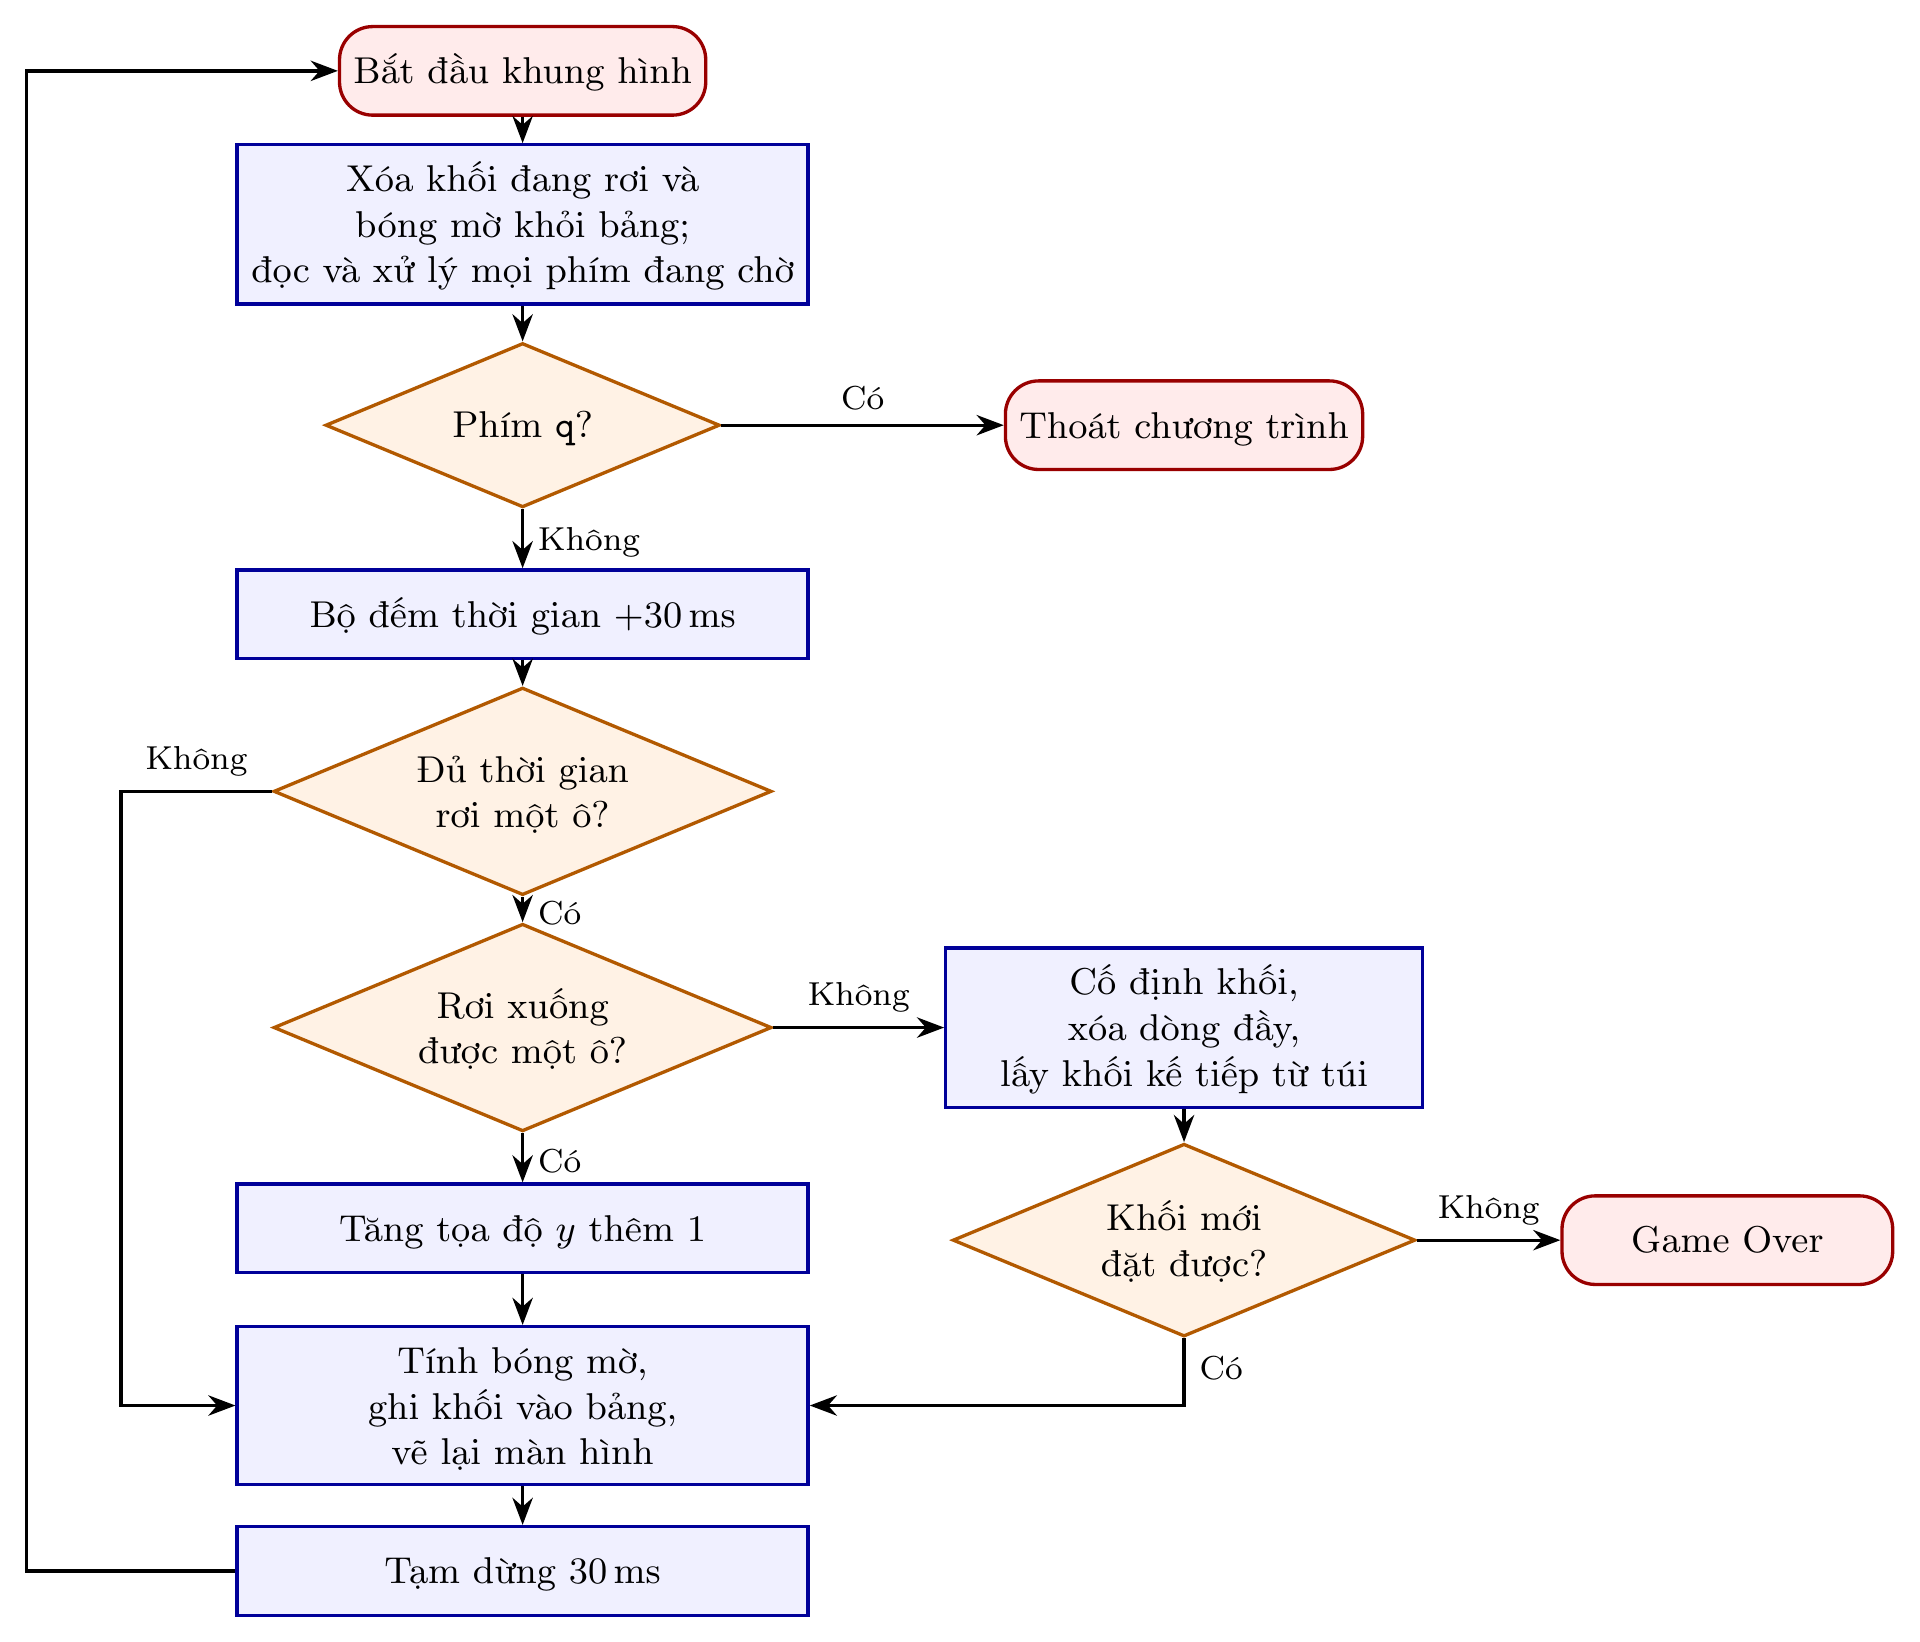
\includegraphics[width=0.72\textwidth]{04_tai_lieu_ky_thuat/so_do/game_loop.png}
    \caption{Lưu đồ xử lý một khung hình trong vòng lặp trò chơi}
    \label{fig:game_loop}
\end{figure}

Các điểm chính trong thiết kế vòng lặp:

\begin{itemize}
    \item \textbf{Xóa trước, vẽ sau}: đầu khung hình, khối đang rơi và bóng mờ được gỡ khỏi bảng, nên khi kiểm tra va chạm, bảng chỉ còn các khối đã cố định. Cuối khung hình, khối được ghi lại ở vị trí mới rồi mới vẽ.
    \item \textbf{Tách tốc độ nhận phím khỏi tốc độ rơi}: phím được đọc mỗi khung hình nên phản hồi nhanh. Khối chỉ tự rơi một ô khi bộ đếm đạt ngưỡng \textit{tốc độ rơi}. Ngưỡng này bắt đầu từ 500\,ms và giảm 50\,ms mỗi cấp, thấp nhất là 50\,ms.
    \item \textbf{Các phím đặc biệt}: Space thả thẳng khối xuống đáy và cố định ngay trong khung hình đó. \texttt{p}/\texttt{Esc} tạm dừng và giữ nguyên trạng thái. \texttt{q} thoát chương trình.
    \item \textbf{Điều kiện kết thúc}: khối mới luôn xuất hiện ở cột 5, hàng 1. Nếu vị trí này đã bị chiếm thì ván chơi kết thúc.
\end{itemize}
